\documentclass[jou]{apa6}

\usepackage[american]{babel}

\usepackage{csquotes}
\usepackage[style=apa,sortcites=true,sorting=nyt,backend=biber]{biblatex}
\DeclareLanguageMapping{american}{american-apa}
\addbibresource{bibliography.bib}


%%%%%%%%%%%%%%%%%%%%%%%%%%%%%%%%%%%%%%%%
%% Discrete Structures
%% The start of RBS stuff
%%%%%%%%%%%%%%%%%%%%%%%%%%%%%%%%%%%%%%%%

% Working internal and external links in PDF
\usepackage{hyperref}
% Extra math symbols in LaTeX
\usepackage{amsmath}
\usepackage{gensymb}
\usepackage{amssymb}
% Enumerations with (a), (b), etc.
\usepackage{enumerate}
\usepackage{xcolor}

\let\OLDitemize\itemize
\renewcommand\itemize{\OLDitemize\addtolength{\itemsep}{-6pt}}

\usepackage{etoolbox}
\makeatletter
\preto{\@verbatim}{\topsep=3pt \partopsep=3pt }
\makeatother

% These sizes redefine APA for A4 paper size
\oddsidemargin 0.0in
\evensidemargin 0.0in
\textwidth 6.27in
\headheight 1.0in
\topmargin -24pt
\headheight 12pt
\headsep 12pt
\textheight 9.19in



\title{Sample Quiz 8}
\author{Discrete Structures, Spring 2020}
\affiliation{RBS}

\leftheader{Discrete Sample Quiz 8}

\abstract{%
}

%\keywords{}

\setlength\parindent{0pt}

\begin{document}

%\thispagestyle{empty}

\twocolumn
\section{Quiz 11: Graphs}

\vspace{4pt}
{\bf Question 1.}
Let $G = (V,E)$ be a graph, where $V$ is the set of all positive divisors of $144$ (including 
$1$ and $144$ itself). Two different vertices $d_1,d_2$ are connected by an edge iff one of the
numbers divides another ($d_1\,\mid\,d_2$ or $d_2\,\mid\,d_1$). 
Find the number of vertices $|V|$ and the number of edges $|E|$ in this graph.

Write two comma-separated integers.


\vspace{10pt}
{\bf Question 2.}
How long is the longest simple circuit in $W_{20}$? 
(A simple circuit is a circular path that may visit vertices multiple times, 
but does not contain any edge more than once.)

Write a positive integer. 




\vspace{10pt}
{\bf Question 3.}
Let $G$ be a planar connected graph with $60$ vertices, each vertex has degree $3$. 
How many regions are there in $G$?

Write a positive integer.



\vspace{10pt}
{\bf Question 4.} This is an adjacency matrix for some graph:
{\footnotesize
$$M_G = \left( 
\begin{array}{ccccccccc}
0 & 1 & 0 & 1 & 0 & 0 & 0 & 0 & 1 \\
1 & 0 & 1 & 1 & 1 & 0 & 0 & 0 & 0 \\
0 & 1 & 0 & 0 & 1 & 1 & 0 & 0 & 0 \\
1 & 1 & 0 & 0 & 1 & 0 & 1 & 0 & 0 \\
0 & 1 & 1 & 1 & 0 & 1 & 1 & 1 & 0 \\
0 & 0 & 1 & 0 & 1 & 0 & 0 & 1 & 1 \\
0 & 0 & 0 & 1 & 1 & 0 & 0 & 1 & 0 \\
0 & 0 & 0 & 0 & 1 & 1 & 1 & 0 & 1 \\
1 & 0 & 0 & 0 & 0 & 1 & 0 & 1 & 0 \\
\end{array} \right).$$
}

It is known that $G$ is a planar graph. Find the number of vertices $|V|$, 
number of edges $|E|$ and the number of regions $|R|$ for this graph. 

Write $3$ comma-separated integers.



\vspace{10pt}
{\bf Question 5 (Dudeney2016, Prob.434), ``536 Puzzles''.}

\begin{figure}[!htb]
\center{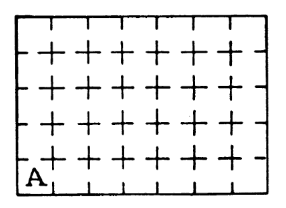
\includegraphics[width=1.5in]{quiz-11/prison-cells.png}}
\caption{\label{fig:prison-cells} A weighted graph.}
\end{figure}

A prisoner currently is in the cell ``$A$'' (Figure~\ref{fig:prison-cells}). He has to visit each 
prison cell no more than once and return 
back to the cell ``$A$''. What is the largest number of prison cells that
can be visited in this way?\\
{\em (Visiting each cell once does not contradict with the requirement to return back 
to ``$A$'' \textendash{} the prisoner uses a circular path between the rooms: 
every room on the path, including ``$A$'', is entered once and left once. We want
to know the maximum length of this path.)}

Write a positive integer.

{\em Note.} You may also want to prove to yourself that the number is the largest possible.


\vspace{10pt}
{\bf Question 6}
There is a bipartite graph $G=(V,E)$ with exactly $|V| = 17$ vertices. (A graph is {\em bipartite}, if 
the set of vertices $V$ can be split into two parts $X$, $Y$ so that all edges are between a vertex in $X$ and a vertex in $Y$.)
Find the largest possible number of edges in such a graph. 

Write a positive integer.
 

\vspace{10pt}
{\bf Question 7} Verify, if these statements are true. 
A simple undirected graph is called a {\em cubic} graph, 
if every vertex has degree $3$.\\
{\bf (A)} There exists a cubic graph with $7$ vertices.\\
{\bf (B)} There exists a cubic graph with $6$ vertices that is not isomorphic to $K_{3,3}$.\\
{\bf (C)} There exists a cubic graph with $8$ edges.

Write a sequence of 3 comma-separated letters (e.g.\ {\tt T,T,T} or {\tt F,F,F}).




\vspace{10pt}
{\bf Question 8.} Verify, if these statements are true:\\
{\bf (A)} There exists a simple directed graph with indegrees $0,1,2,4,5$ and outdegrees $0,3,3,3,3$. (A graph is {\em simple}, if
it is not a {\em multigraph} \textendash{} there is no more than one edge $(u,v)$ for any vertices $u,v$.)\\
{\bf (B)} There exists a connected undirected simple planar graph with $5$ regions and $8$ vertices, each vertex has degree $3$.\\
{\bf (C)} There exists a connected undirected simple planar graph with $8$ regions and $6$ vertices, each region is surrounded 
with $3$ edges.

Write a sequence of 3 comma-separated letters (e.g.\ {\tt T,T,T} or {\tt F,F,F}).



\vspace{10pt}
{\bf Question 9.}
Use Dijkstra’s Algorithm to find the shortest paths from the source vertex $s$ 
to all other vertices $t,x,y,z$ (Figure~\ref{fig:dijkstra}). The length of a path is obtained by adding the 
weights of the directed edges.

\begin{figure}[!htb]
\center{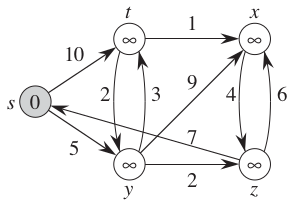
\includegraphics[width=1.8in]{quiz-11/dijkstra.png}}
\caption{\label{fig:dijkstra} A weighted graph.}
\end{figure}


Write $4$ comma-separated numbers \textendash{} the shortest paths 
to the vertices $t,x,y,z$ respectively.

{\em Note.} Dijkstra's algorithm (Rosen2019, p.747) initializes the set of vertices $S$ that we 
know the shortest paths to (initially it only contains the 
source vertex $S = \{ s \}$; 
the distance from $s$ to itself is $0$; initialize the distances to 
all the other vertices to $\infty$). At every step consider all the edges that 
go from the set $S$ to $\overline{S}$, i.e. to the vertices where we still 
do not know the shortest paths. Update all the shortest paths (if crossing from 
the set $S$ to $\overline{S}$ finds a shorter path than $\infty$ or the currently 
known minimum length, then decrease the estimate for this vertex). 
Finally, add the minimum vertex from $\overline{S}$ to $S$. Repeat the steps
until all vertices are added to $S$ and all the shortest path estimates have 
reached their smallest values.





\vspace{10pt}
{\bf Question 10 (Dudeney2016, Prob.423), ``536 Puzzles''.}
A man starting from the town $A$, has to inspect all the roads
shown from town to town (Figure~\ref{fig:path-with-repetitions}). 
Their respective lengths, $13$, $12$, and $5$
miles are all shown. What is the shortest possible route he can adopt, 
ending his journey wherever he likes?

\begin{figure}[!htb]
\center{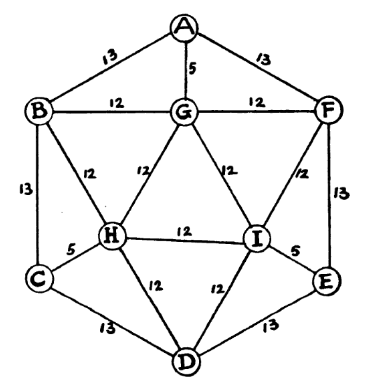
\includegraphics[width=2in]{quiz-11/path-with-repetitions.png}}
\caption{\label{fig:path-with-repetitions} Path with repetitions}
\end{figure}

Write an integer \textendash{} the length of the shortest route.

{\em Note.} This graph obviously has no Euler path (since there
are more than $2$ vertices with odd degrees). The problem is to 
find a path that is likely {\bf not} simple 
(uses the same edge several times), 
but that includes every edge shown and the total of weights is minimal. 





\vspace{10pt}
{\bf Question 11}\\
Somebody placed $24$ chess rooks on a $8 \times 8$ chessboard as shown in Figure~\ref{fig:rooks}
(each horizontal and each vertical has exactly $3$ rooks). 


\begin{figure}[!htb]
\center{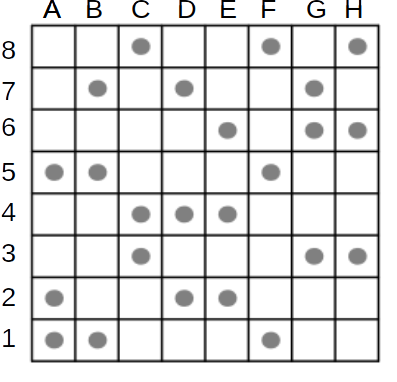
\includegraphics[width=1.5in]{quiz-11/rooks.png}}
\caption{\label{fig:rooks} Path with repetitions}
\end{figure}

We imagine that this chess-board defines a bipartite graph between the  
set of all verticals $X= \{ A,B,C,D,E,F,G,H \}$ and the set of all 
horizontals $Y= \{ 1,2,3,4,5,6,7,8 \}$. Any rook defines an edge between these two sets. 
For example, the rook $C8$ defines an edge $(C,8)$. 

Find a subset of verticals $V \subseteq X$ such that $|V|=3$, but
the neighbor set has size $|N(V)| = 5$.

Write $3$ comma-separated letters in your answer (the vertices from $V$). It is 
sufficient to write just one possible answer, if there are many.

\vspace{10pt}
{\em Note 1.} For example, the answer $\textcolor{blue}{\mathtt{F,G,H}}$ does not work, 
since the set of vertices $\{ \mathtt{F},\mathtt{G},\mathtt{H} \} \subseteq X$ 
is neighboring with a set of six vertices
$\{ 1,3,5,6,7,8 \} \subseteq Y$, i.e. the rooks on these three verticals
attack six horizontals, but not five.

{\em Note 2.} For the condition of the Hall's marriage theorem we need the inequality $|V| \leq |N(V)|$ 
for {\bf every} $V \subseteq X$. You could prove to yourself that it is always satisfied
(also for all the other placements of $24$ rooks where each horizontal and each 
vertical has $3$ rooks).\\
{\em Note 3.} Interpret for yourself what does a ``perfect matching'' between the sets
$X$ and $Y$ mean in this subject-area with a chessboard and rooks.




\newpage

\subsection{Answers}


\vspace{4pt}
{\bf Question 1} Answer: $15,75$\\
Since $144 = 2^4 \cdot 3^2$, number $144$ has $(4+1)(2+1) = 15$ divisors
(the number of ways to pick powers $2^a \cdot 3^b$). 
Their Hasse diagram is shown in Figure~\ref{fig:divisibility-144-graph}
(transitive closure has many more arrows that are not shown). 

For each vertex $d_1$ we calculate the number of other vertices that
are divisible by $d_1$ (i.e. can be reached by following one or more arrows in the
Hasse diagram). Adding all those numbers gives the number of edges.

\begin{figure}[!htb]
\center{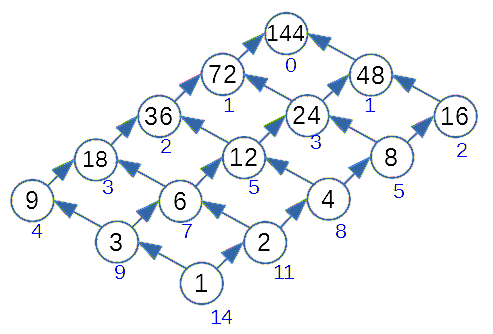
\includegraphics[width=3in]{quiz-11/divisibility-144-graph.png}}
\caption{\label{fig:divisibility-144-graph} Divisibility Hasse diagram.}
\end{figure}




\vspace{10pt}
{\bf Question 2} Answer: $30$\\
All the vertices on the regular $20$-gon have degree equal to $3$. 
This means that we have to drop at least $10$ edges before we 
get a simple path (because any simple path adds only even number to the degree
of any vertex in a graph). Initially $W_{20}$ has $20 + 20 = 40$ edges. 
After deleting $10$ edges (every other edge on the perimeter of the $20$-gon), 
we are left with $30$ edges.


\vspace{10pt}
{\bf Question 3} Answer: $32$\\
$60$ vertices (having degree $3$ each would create the sum of all degrees equal to $60 \cdot 3 = 180$. 
The number of edges equals one half of that; so $|E| = 90$. The number of regions
can be computed using Euler's formula: $|V| - |E| + |R| = 2$ (in our case 
$60 - 90 + |R| = 2$; therefore $|R| = 32$. 

One example of such graph is {\em truncated icosahedron}, see \url{https://bit.ly/2WaSW6I}, 
but there may be many others that are not isomorphic to it. Still, all of them 
would have the same number of regions due to Euler's formula.

\vspace{10pt}
{\bf Question 4} Answer: {\tt 9,17,10}\\
Number of vertices equals the size of the matrix $9 \times 9$, 
so $|V| = 9$. The number of edges is one half of all the $1$s written 
in the adjacency matrix; therefore $|E| = 17$. Since we can assume
that the graph $G$ is planar, it satisfies Euler's formula:
$$|V| - |E| + |R| = 2.$$
Therefore the number of regions $|R| = 10$. 

Graph (shown without edge intersections as a planar graph) is visible 
on Figure~\ref{fig:question4-graph}. In this picture we can simply count 
vertices, edges and regions. But it is usually time-consuming to 
create such pictures (and to verify that they match the adjacency matrix).

\begin{figure}[!htb]
\center{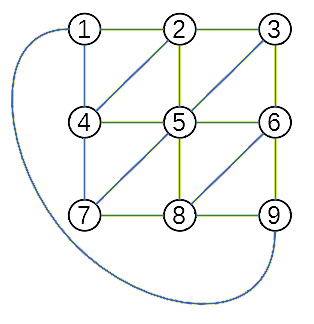
\includegraphics[width=1.5in]{quiz-11/question4-graph.png}}
\caption{\label{fig:question4-graph} A planar graph}
\end{figure}


\vspace{10pt}
{\bf Question 5} Answer: $34$\\
It is easy to build a path that visits all rooms except one. 
There cannot be a circular path with exactly $35$ steps \textendash{}
one can use checkerboard pattern (color all cells in black and white). 
Every step switches the color to the opposite; after exactly $35$ color switches
the color would be opposite \textendash{} the path cannot return back to cell $A$.


\vspace{10pt}
{\bf Question 6} Answer: $72$\\
We know that the sum of two sizes $|X| + |Y| = 17$, 
and the maximum number of edges is $|X| \cdot |Y|$. 
The greatest possible product of two numbers is
when they are closest to each other: 
$8 \cdot 9 = 72$. (We can try out all combinations of two numbers
that add up to $17$ to see that this is the largest one.)

We can write the following algebraic inequalities: 
$$|X| \cdot |Y| \leq \left( \frac{|X| + |Y|}{2} \right)^2,$$
$$4 |X| \cdot |Y| \leq \left( |X| + |Y| \right)^2,$$
$$4 |X| \cdot |Y| \leq |X|^2 + |Y|^2 + 2 |X| \cdot |Y|,$$
$$0 \leq |X|^2 + |Y|^2 = 2 |X| \cdot |Y| = (|X| + |Y|)^2.$$

From the first inequality we imply that $|X| \cdot |Y| \leq (17/2)^2 = 72.25$. 
Since the number of edges cannot be fractional, $72$ is indeed the largest number.



\vspace{10pt}
{\bf Question 7} Answer: {\tt FTT}\\
{\bf (A)} False. No cubic graph can have odd number of vertices 
(the sum of all degrees of all vertices should be even \textendash{} twice the number of edges).\\
{\bf (B)} True. $K_{3,3}$ is bipartite graph (it does not contain any ``triangles'': three vertices
that are all mutually connected). But the graph on Figure~\ref{fig:cubic-graph-6}
is not bipartite (so it is not isomorphic
to $K_{3,3}$.

\begin{figure}[!htb]
\center{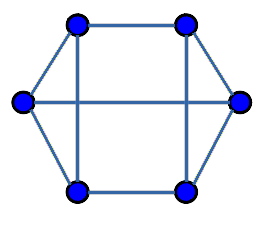
\includegraphics[width=1in]{quiz-11/cubic-graph-6.png}}
\caption{\label{fig:cubic-graph-6} Cubic graph with 6 vertices.}
\end{figure}

{\bf (C)} True. You can draw a regular octagon and add all the long diagonals. 
Now every vertex is adjacent with three vertices (both neighbors and the opposite one). 


\vspace{10pt}
{\bf Question 8} Answer: {\tt FFT}\\
{\bf (A)} False. In a simple directed graph with $5$ vertices, an indegree 
$5$ means that all vertices should point arrows to the given vertex (including the vertex itself). 
But in this case there cannot be any vertices with outdegree $0$.\\
{\bf (B)} False. A graph with $8$ vertices of degree $3$ means that it has $\frac{8 \cdot 3}{2} = 12$ edges. 
According to Euler's formula, the number of regions should be $R = 2 + E - V = 6$. Therefore 
such a graph should have $6$ (not $5$) regions.\\
{\bf (C)} True. Such graph exists. For example Octahedron - see \url{https://bit.ly/3f1gnrG}.



\vspace{10pt}
{\bf Question 9} Answer: {\tt 8,9,5,7}

{\footnotesize
\begin{tabular}{|l|l|l|} \hline
Set $S$ & Weights of $\overline{S}$ & Added to $S$ \\ \hline
$\{ s \}$ & $w(t,x,y,z) = (10,\infty,5,\infty)$ & $y$ (min path $5$) \\  \hline
$\{ s,y \}$ & $w(t,x,z) = (8,\infty,7)$ & $z$ (min path $7$) \\ \hline
$\{ s,y,z \}$ & $w(t,x) = (8,9)$ & $t$ (min path $8$) \\ \hline
$\{ s,t,y,z \}$ & $w(x) = 9$ & $x$ (min path $9$) \\ \hline
\end{tabular}
}


\vspace{10pt}
{\bf Question 10} Answer: {\tt 211}\\
There are altogether $6$ vertices with odd degrees (one of them is $A$). If we start our travel in $A$
and end it in any other vertex with odd degree (say, in $G$), then there are 
four more vertices with odd degrees. By adding edges $(C,H)$ and $(I,E)$ two times, we can 
build the required path (each of these edges has weight $5$). Therefore the full length of the 
path is the sum of all weights: 
$$3 \cdot (12 + 12 + 12) + 3 \cdot (13 + 13 + 5) + (5 + 5).$$

\begin{figure}[!htb]
\center{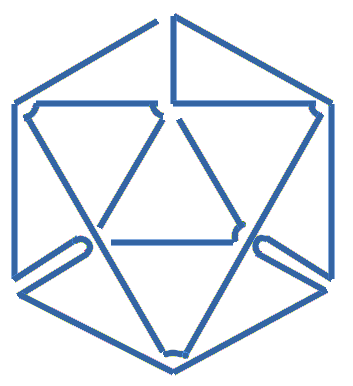
\includegraphics[width=1.5in]{quiz-11/path-with-repetitions2.png}}
\caption{\label{fig:path-with-repetitions2} Path with Repetitions (Solved).}
\end{figure}


\vspace{10pt}
{\bf Question 11} Answer: {\tt "A,B,D"}, {\tt "A,B,F"}, 
{\tt "C,E,H"}, {\tt "C,G,H"}, {\tt "D,E,G"}\\
There are five ways to select the verticals (any one of them is correct). 
Since the rooks (as edges linking horizontals with verticals) satisfy the Hall's Marriage theorem, 
there exists a perfect matching: One can select $8$ rooks (out of the $24$) so that
each rook has its own horizontal and its own vertical. In other words, they do not attack each other. 

We can start searching this perfect matching using ``backtracking'' \textendash{} first 
try to pick the minimum possible horizontal in each vertical (avoiding any attacking position). 
If this leads in a dead end, then start moving the rooks that have been placed last. 
This very quickly leads to a solution (Figure~\ref{fig:rooks2}). There are also many other 
perfect matchings.

\begin{figure}[!htb]
\center{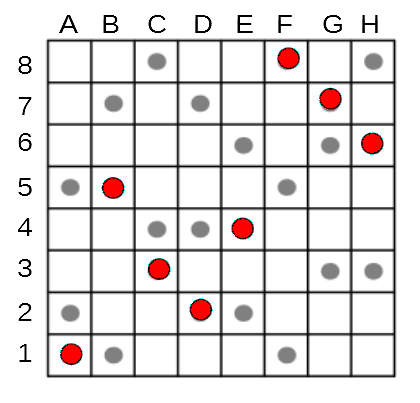
\includegraphics[width=1.5in]{quiz-11/rooks2.png}}
\caption{\label{fig:rooks2} 8 selected rooks shown red}
\end{figure}




\end{document}

